\begin{abstract}
Federated learning (FL) lets a small group of malicious clients plant a hidden trigger-to-target behaviour in the shared model. A behavioural defence probes each client's candidate model directly: it stamps patches on a small clean server set and measures how often predictions flip to a class. We study one such defence, ProbeGuard, and ask a narrow question: when detection weakens under non-IID data, is the \emph{score} to blame or the \emph{rule} that thresholds it? We examine this on a controlled digits/MLP benchmark (20 clients, 20\% attackers, 20 seeds). A median-absolute-deviation (MAD) rule leaves the final attack success rate (ASR) at 86\%, 71\%, 46\% and 0.7\% for Dirichlet $\alpha=0.1,0.5,1,10$, against 86--69\% for plain averaging, even though the score keeps real ranking power: its closed-loop late-round AUROC is 0.81 at $\alpha=0.5$ and 0.93 at $\alpha=1$. Across nine $\alpha$ values, the benign score spread correlates negatively with the MAD detection rate ($r=-0.81$). A rank-based rule that drops the $f$ highest scores each round cuts ASR to 34\% ($\alpha=0.5$) and 7.6\% ($\alpha=1$), and a smaller fixed MAD multiplier recovers most of the same gain (20 seeds), so the loss is largely one of calibration. Both pay a false-positive cost, the rank rule requires $f$ in advance, and neither helps at $\alpha=0.1$. Coordinate median and FLTrust remain stronger at low $\alpha$. A probe-aware adaptive attacker raises the rank rule's ASR at $\alpha=1$ from 7\% to 12\%, and a CIFAR-10 CNN check (8 seeds, $\alpha=10$) finds both rules within about half a point of an oracle but does not test heterogeneity at that scale.
\end{abstract}
\begin{IEEEkeywords}
federated learning, backdoor attacks, model inspection, non-IID data, decision rules, trustworthy machine learning
\end{IEEEkeywords}

\section{Introduction}
Federated learning (FL) trains one model across many data holders without moving their raw data \cite{mcmahan2017}. The same openness lets a minority of participants insert a backdoor: behaviour that stays quiet on clean inputs and fires when a chosen pattern is present. Recent surveys catalogue a wide range of such attacks and of defences against them \cite{li2025survey}. Defences either analyse the geometry of client updates, as in the classic median, trimmed-mean and Krum rules \cite{blanchard2017,yin2018}, anchor trust in a server dataset \cite{cao2021}, or inspect the submitted models themselves \cite{rieger2022,nguyen2022,rieger2024,zhang2025}.

Statistical heterogeneity complicates all of these. When client data are non-IID, learning itself becomes harder \cite{li2022niid} and honest updates already disagree with one another, so the boundary between benign and malicious behaviour is blurred. Defence papers usually report one heterogeneity level and read a failure as a failure of the detector. That conflates two causes with different remedies: the score may carry no information, or it may carry plenty while the threshold is badly matched to the spread of benign scores.

We separate the two using a flip-rate probe score (ProbeGuard) as the test case. We do not propose a stronger detector; we ask where the loss occurs. Our contributions are:
\begin{itemize}
\item a split of \emph{score quality} (AUROC) from \emph{decision quality} (TPR, FPR, ASR) across eight heterogeneity levels, 20 seeds;
\item a median-containment argument for the score and a measured link from heterogeneity to benign score spread to MAD detection rate;
\item a comparison of decision rules on one score (MAD at several multipliers, percentiles, a rank-based top-$f$ rule, an oracle), including the cost of misjudging $f$;
\item a probe-aware adaptive attacker, a CIFAR-10 CNN check, and what did not work.
\end{itemize}
We claim neither state-of-the-art accuracy, optimal-adversary robustness, nor generality across trigger families.

\section{Related Work}
Robust aggregation includes Krum and Multi-Krum \cite{blanchard2017} and coordinate-wise median and trimmed mean \cite{yin2018}; FLTrust derives trust from a clean server root set \cite{cao2021}. Later defences inspect model behaviour or structure: DeepSight and FLAME \cite{rieger2022,nguyen2022} screen updates beyond simple distances, CrowdGuard \cite{rieger2024} analyses hidden-layer outputs of local models on other clients' data and is evaluated under non-IID splits, FreqFed \cite{fereidooni2024} works on a frequency-domain view of the updates, Lockdown \cite{huang2023} isolates client training subspaces and prunes, and a representation-dissimilarity detector \cite{zhang2025} excludes outlying clients iteratively. AlignIns \cite{xu2025} inspects update directions, noting that benign non-IID updates perturb pairwise similarity, and FilterFL \cite{yang2025} synthesises trigger-like samples without auxiliary data for extreme heterogeneity. Trigger inversion \cite{xu2024} recovers a trigger from a model already known to be backdoored. ProbeGuard sits closest to CrowdGuard and to trigger probing: it feeds fixed candidate triggers to each client model on a server-held clean set and scores the flip response. We do not claim it beats these methods and did not compare against them; the contribution is an analysis of how its score and rule behave as heterogeneity changes.

\section{Method}
\subsection{Setting and Threat Model}
Of $n$ clients, a set $\mathcal M$ with $|\mathcal M|=m<n/2$ is malicious. In round $t$ client $i$ returns an update $u_i$ computed from the server model $w_t$. Malicious clients stamp a trigger $\tau$ on a fraction $\rho$ of their non-target samples and relabel them with the target class. The server keeps a small clean root set $D_0$ and sets $w_{t+1}=w_t+\mathrm{Agg}(u_1,\dots,u_n)$. The goal is a low ASR (share of triggered non-target test inputs classified as the target) at unchanged clean accuracy.

The attacker can poison local data, control fewer than half of the clients, and knows the target class and trigger. In the main experiments the attacker does \emph{not} know that ProbeGuard is deployed and does not optimise against its score; Section~\ref{sec:adaptive} relaxes this.

\subsection{Probe Score}
Let $\mathcal B$ be the bank of all $2{\times}2$ saturated patches at the 49 positions of an $8{\times}8$ image. For candidate model $f_i=f(w+u_i)$, patch $p$ and class $c$, the flip rate is
\begin{equation}
R_i[p,c]=\frac{\#\{x\in D_0:\ y(x)\neq c,\ f_i(\mathrm{stamp}_p(x))=c\}}{\#\{x\in D_0:\ y(x)\neq c\}}.
\end{equation}
With $\tilde R$ the cellwise median over clients, the client score is $s_i=\max_{p,c}\,(R_i[p,c]-\tilde R[p,c])$. The probe size matches the fixed, multi-location and low-intensity triggers, so those have a matching probe cell; the $3{\times}3$ trigger deliberately has none.

\begin{figure}[t]
\centering
\begin{tikzpicture}[font=\scriptsize,
 box/.style={draw,rounded corners=1.5pt,align=center,minimum height=7mm,inner sep=2pt,text width=23mm},
 arr/.style={-{Latex[length=1.6mm]},line width=0.5pt}]
\node[box,fill=gray!10] (cl) at (0,0) {Client updates $u_i$ (benign and malicious)};
\node[box,fill=gray!10] (cand) at (2.95,0) {Candidate models $w_t{+}u_i$};
\node[box,fill=orange!12] (probe) at (5.9,0) {Probe bank: 49 patches on root set $D_0$};
\node[box,fill=orange!12] (rate) at (5.9,-1.2) {Flip rates $R_i[p,c]$};
\node[box,fill=green!10] (score) at (2.95,-1.2) {Score $s_i$: max excess over median $\tilde R$};
\node[box,fill=green!10] (rule) at (0,-1.2) {Decision rule: MAD or top-$f$};
\node[box,fill=gray!10] (agg) at (0,-2.4) {Average the kept updates};
\draw[arr] (cl)--(cand); \draw[arr] (cand)--(probe); \draw[arr] (probe)--(rate);
\draw[arr] (rate)--(score); \draw[arr] (score)--(rule); \draw[arr] (rule)--(agg);
\end{tikzpicture}
\caption{ProbeGuard per round: each candidate model is probed with a bank of patches on the server's clean root set; the flip-rate tensor is compared with the cross-client median, and a decision rule excludes clients before averaging.}
\label{fig:pipe}
\end{figure}
\subsection{Decision Rules}
All rules act on the same scores $s_i$. The \emph{MAD rule} flags client $i$ if $s_i>\mathrm{med}(s)+\max(k\cdot\mathrm{MAD}(s),\delta)$. \emph{Percentile rules} flag scores above a fixed percentile of the round's scores. The \emph{top-$f$ rule} (ProbeGuard-K) removes the $f$ highest scores each round; like Multi-Krum it is given $f$. An \emph{oracle threshold} uses the true labels and serves only as a ceiling. The server averages the updates that remain.

\subsection{Why the Score Separates Clients}
\begin{lemma}[Median containment]
If $m<n/2$, then for every cell $\min_{j\notin\mathcal M}R_j[p,c]\le\tilde R[p,c]\le\max_{j\notin\mathcal M}R_j[p,c]$.
\end{lemma}
\begin{proof}
Take a middle order statistic $v$ of the $n$ values in a cell. At least $\lceil n/2\rceil>m$ values are at most $v$, so one of them is benign; the same holds above $v$. The median equals $v$ or averages the two middle values, so it lies between the smallest and largest benign values.
\end{proof}
\begin{proposition}[Score separability]
Let $\Delta_B=\max_{p,c}\bigl(\max_{j\notin\mathcal M}R_j[p,c]-\min_{j\notin\mathcal M}R_j[p,c]\bigr)$ be the benign spread. Every benign client has $s_j\le\Delta_B$, and a malicious client with trigger cell $(p^*,c^*)$ has $s_i\ge R_i[p^*,c^*]-\max_{j\notin\mathcal M}R_j[p^*,c^*]$. Hence all malicious scores exceed all benign scores whenever the trigger response beats the benign maximum in its cell by more than $\Delta_B$.
\end{proposition}
The upper bound on $s_j$ uses $\tilde R\ge\min_{j\notin\mathcal M}R_j$ and the lower bound on $s_i$ uses $\tilde R\le\max_{j\notin\mathcal M}R_j$, both from the lemma. The condition is sufficient only and holds round by round, but it names the mechanism: $\Delta_B$ grows when benign models respond differently to saturated patches, which class-skewed models do because they lean toward their dominant classes. The result concerns scores, not the thresholded rule, which also depends on $\mathrm{MAD}(s)$ and on the state of the model early in training. We never measure $\Delta_B$ itself; Section~\ref{sec:mech} uses the standard deviation of benign scores as a proxy.
\begin{proposition}[Rank rule under separability]
In a round where every malicious score exceeds every benign score (ties excluded), suppose the server drops the $f$ highest scores. If $f\ge m$, all $m$ malicious updates are removed and at most $f-m$ benign updates are discarded. If $f<m$, exactly $m-f$ malicious updates remain, a share $(m-f)/(n-f)$ of the average, which is below the unfiltered share $m/n$.
\end{proposition}
\begin{proof}
The $f$ highest scores are malicious until the $m$ malicious clients are exhausted, which gives both cases. Since $n>m$ and $f>0$, $n(m-f)<m(n-f)$, so $(m-f)/(n-f)<m/n$.
\end{proof}
This matches the misspecification results below: under-estimating $f$ leaves attackers in, over-estimating it discards benign clients.

\section{Experimental Setup}
\textbf{Data and model.} We use the scikit-learn digits set (1,797 images of $8{\times}8$ pixels) \cite{pedregosa2011}, split per seed into 1,200 training, 100 server-root and 497 test images. The model is a 64--32--10 ReLU MLP written in NumPy \cite{harris2020} and trained with SGD (learning rate 0.1, batch 32, two local epochs). There are $n=20$ clients, 30 rounds, full participation, and Dirichlet label-skew partitions \cite{li2022niid}.

\textbf{Attacks.} The target class is 0. By default $m=4$ clients (20\%) poison half of their non-target samples, without update boosting. Fixed ($2{\times}2$, intensity 1, bottom-right), multi-location, low-intensity and $3{\times}3$ triggers are used; ASR is measured with the matching trigger.

\textbf{Baselines.} FedAvg, coordinate median and 20\% trimmed mean \cite{yin2018}, norm clipping to the median update norm, Multi-Krum \cite{blanchard2017} (given the true $f$), FLTrust \cite{cao2021}, and a benign-only oracle. These are our own simplified implementations.

\textbf{Seed sets.} \emph{Study B} (seeds 100--119; $\alpha\in\{0.1,0.25,0.5,0.75,1,1.5,2,5\}$, plus $\alpha=10$ in a separate run) runs FedAvg, the MAD rule and the top-$f$ rule on 20 seeds and contains the $f$-sensitivity runs. The baseline comparison, the decision-rule sweep and the adaptive attacker were re-run on the same 20 seeds. \emph{Study A} (seeds 0--7) still supplies the open-loop AUROC analysis, the spread study and the CNN test; its original scripts were not preserved, so those results are indicative. The MAD parameters ($k{=}2$, $\delta{=}0.1$) were chosen on seeds 100--102 at $\alpha=1$, which are also in Study B; dropping them changes the $\alpha=1$ means only slightly (MAD 44.4\% vs 46.4\%, top-$f$ 4.0\% vs 7.6\%).

\textbf{Statistics.} We report means with 95\% percentile-bootstrap intervals (10,000 resamples), which respect the $[0,1]$ range of ASR, and paired exact Wilcoxon tests with Holm correction, computed with SciPy \cite{virtanen2020}. With few seeds, non-significance is not equivalence.

\section{Results}
\subsection{Heterogeneity and Baselines}
Table~\ref{tab:base} shows how the MAD rule compares with other defences. At $\alpha=10$ it reaches 0.7\% ASR at 89.6\% clean accuracy (oracle 89.7\%), against 69.1\% for FedAvg. As $\alpha$ falls the picture changes: 46.4\% at $\alpha=1$, and at $\alpha\le0.5$ it is barely better than averaging. Coordinate median and FLTrust are far better in that regime, although the median pays for it in accuracy (50.1\% clean accuracy at $\alpha=0.1$ versus 80.5\% for ProbeGuard). The probe-based defence is therefore not the strongest option under strong heterogeneity.
\begin{table}[t]
\caption{Study A: ASR (\%) with the fixed trigger, 20\% malicious clients, mean over 20 seeds.}
\label{tab:base}
\centering\footnotesize
\begin{tabular}{@{}lcccc@{}}
\toprule
Defence & $\alpha{=}0.1$ & $\alpha{=}0.5$ & $\alpha{=}1$ & $\alpha{=}10$\\
\midrule
FedAvg & 86.0 & 77.8 & 74.9 & 69.1\\
Coord.\ median & 24.3 & 7.0 & 3.5 & 1.2\\
Trimmed mean & 38.4 & 9.0 & 4.6 & 1.9\\
Norm clipping & 85.7 & 73.4 & 67.9 & 34.2\\
Multi-Krum & 85.0 & 55.3 & 40.9 & 10.4\\
FLTrust & 35.9 & 9.8 & 1.7 & 0.7\\
ProbeGuard (MAD) & 86.5 & 70.7 & 46.4 & 0.7\\
Oracle (benign only) & 0.4 & 0.3 & 0.3 & 0.3\\
\bottomrule
\end{tabular}
\end{table}

Table~\ref{tab:b} and Fig.~\ref{fig:alpha} give the 20-seed view (Study B). Between $\alpha=0.5$ and $\alpha=2$ the MAD rule removes only a fraction of the attackers (cumulative TPR 0.06 at $\alpha=0.5$, 0.22 at $\alpha=1$), while its false-positive rate stays near 0.02. It is no better than FedAvg at $\alpha\le0.25$ and approaches the top-$f$ rule only for $\alpha\ge5$ (Holm-adjusted $p=0.18$ there).

\begin{figure*}[t]
\centering
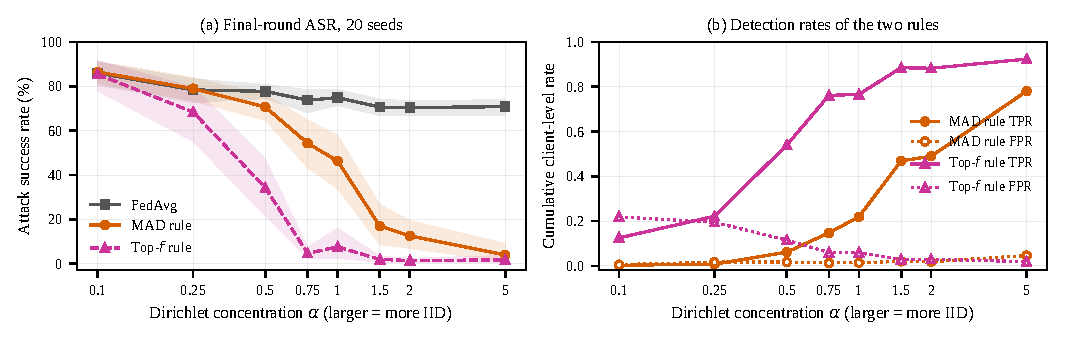
\includegraphics[width=\textwidth]{figs/fig_alpha.pdf}
\caption{Study B (20 seeds, fixed trigger, 20\% malicious). (a) Final-round ASR against heterogeneity; bands are 95\% bootstrap intervals. (b) Cumulative client-level TPR (solid) and FPR (dotted) of the two decision rules computed on the same score.}
\label{fig:alpha}
\end{figure*}

\begin{table*}[t]
\caption{Study B: final ASR (\%) with 95\% bootstrap interval, cumulative client-level TPR/FPR, and clean accuracy (\%); 20 seeds, fixed trigger. $\Delta$ is top-$f$ minus MAD in percentage points; $p$ is the paired Wilcoxon p-value with Holm correction over all 24 sweep comparisons.}
\label{tab:b}
\centering\footnotesize\setlength{\tabcolsep}{3.2pt}
\begin{tabular}{@{}lccccccccc@{}}
\toprule
 & \multicolumn{3}{c}{ASR (\%) [95\% CI]} & \multicolumn{2}{c}{Top-$f$ vs.\ MAD} & \multicolumn{2}{c}{TPR/FPR} & \multicolumn{2}{c}{Clean acc.\ (\%)}\\
\cmidrule(lr){2-4}\cmidrule(lr){5-6}\cmidrule(lr){7-8}\cmidrule(lr){9-10}
$\alpha$ & FedAvg & MAD & Top-$f$ & $\Delta$ & $p_\text{Holm}$ & MAD & Top-$f$ & FedAvg & Top-$f$\\
\midrule
0.1 & 86.0 [80.6, 90.9] & 86.5 [81.4, 91.2] & 85.4 [77.8, 91.6] & -1.0 & 1.00 & 0.00/0.01 & 0.12/0.22 & 81.2 & 76.0\\
0.25 & 78.4 [72.7, 83.4] & 79.0 [73.4, 84.0] & 68.4 [55.2, 79.6] & -10.6 & 1.00 & 0.01/0.02 & 0.22/0.19 & 87.1 & 84.7\\
0.5 & 77.8 [74.5, 80.9] & 70.7 [64.7, 76.3] & 34.2 [21.5, 47.2] & -36.5 & $<$0.001 & 0.06/0.02 & 0.54/0.12 & 88.2 & 88.2\\
0.75 & 73.8 [68.2, 78.5] & 54.3 [43.2, 64.9] & 4.7 [2.5, 7.4] & -49.6 & $<$0.001 & 0.15/0.01 & 0.76/0.06 & 88.3 & 88.9\\
1 & 74.9 [71.4, 78.6] & 46.4 [33.9, 58.1] & 7.6 [2.4, 16.0] & -38.8 & $<$0.001 & 0.22/0.01 & 0.77/0.06 & 88.6 & 89.6\\
1.5 & 70.7 [66.9, 74.2] & 17.0 [8.7, 26.6] & 1.9 [0.7, 3.5] & -15.0 & $<$0.001 & 0.47/0.02 & 0.89/0.03 & 88.9 & 90.1\\
2 & 70.5 [67.0, 73.5] & 12.6 [6.9, 19.5] & 1.5 [0.7, 2.4] & -11.1 & $<$0.001 & 0.49/0.02 & 0.88/0.03 & 89.0 & 89.7\\
5 & 70.8 [67.0, 74.1] & 3.9 [1.0, 9.1] & 1.7 [0.4, 3.7] & -2.2 & 0.18 & 0.78/0.05 & 0.92/0.02 & 88.6 & 89.8\\
\bottomrule
\end{tabular}
\end{table*}

\subsection{Score Quality Versus Decision Quality}
\textbf{Open-loop separability (Study A).} To ask whether the score or the rule fails, we logged scores along trajectories of a benign-only global model (19,200 client-round scores) and computed threshold-free AUROC over rounds 16--30: $0.72\pm0.06$ ($\alpha=0.1$), $0.949\pm0.020$ (0.5), $0.978\pm0.012$ (1) and $0.993\pm0.008$ (10), as 95\% intervals over seeds. Early rounds (1--5) are weaker for small $\alpha$ (0.57, 0.83, 0.92, 0.99) as the local backdoor has not yet formed. AUPRC, which accounts for the 20\% base rate, tracks AUROC (0.34, 0.82, 0.93, 0.96). In this setting the score is informative at $\alpha\in\{0.5,1\}$ while the MAD rule is poor.

\textbf{Closed-loop separability (Study B).} In instrumented 20-seed runs where the defence's own decisions shape the global model, late-round AUROC of the MAD runs is lower: $0.81$ at $\alpha=0.5$ and $0.93$ at $\alpha=1$. Part of the gap may arise because early misses let the global model absorb the backdoor, so malicious updates stand out less; we did not isolate this effect. Per seed, late-round AUROC and final ASR are strongly related (Spearman $\rho=-0.82$ at $\alpha=0.5$ and $-0.84$ at $\alpha=1$, $n=20$ each; Fig.~\ref{fig:mech}b), so seeds on which the score separates poorly are also the seeds on which the defence fails.

\textbf{Percentile rules.} Table~\ref{tab:rules} applies other rules to the identical score. Fixed percentile thresholds do not help: at $\alpha=0.1$ all stay within a few points of FedAvg, and everywhere they stay far above the oracle (38--58\% at $\alpha=10$). Among the rules in Table~\ref{tab:rules}, only top-$f$ comes close to the oracle at $\alpha\ge1$; Section~\ref{sec:calib} shows that a smaller MAD multiplier closes most of the same gap.
\begin{table}[t]
\caption{ASR (\%) of different decision rules on the same score, 20 seeds, fixed trigger.}
\label{tab:rules}
\centering\footnotesize
\begin{tabular}{@{}lcccc@{}}
\toprule
Decision rule & $\alpha{=}0.1$ & $\alpha{=}0.5$ & $\alpha{=}1$ & $\alpha{=}10$\\
\midrule
FedAvg (no rule) & 86.0 & 77.8 & 74.9 & 69.1\\
MAD, $k{=}2$ & 86.5 & 70.7 & 46.4 & 0.7\\
MAD, $k{=}1$ & 86.2 & 43.6 & 11.1 & 0.3\\
90th percentile & 86.8 & 66.2 & 47.7 & 38.3\\
95th percentile & 86.7 & 72.7 & 65.3 & 58.0\\
97.5th percentile & 86.7 & 72.7 & 65.4 & 58.1\\
Top-$f$ (true $f$) & 85.4 & 34.2 & 7.6 & 0.8\\
Oracle threshold & 0.4 & 0.3 & 0.3 & 0.3\\
\bottomrule
\end{tabular}
\end{table}

\subsection{Mechanism: Benign Score Spread}\label{sec:mech}
Proposition~1 predicts that detection should suffer where the benign spread is large. Over nine $\alpha$ values from 0.1 to 10, the mean standard deviation of benign scores is 0.15--0.17 for $\alpha\le0.5$ and about 0.12 for $\alpha\ge2$, with a sharp drop between $\alpha=0.5$ and $\alpha=1$; the dependence is not strictly monotone (the maximum, 0.172, is at $\alpha=0.3$). This spread is negatively related to the MAD rule's TPR ($r=-0.81$, $n=9$, $p=0.009$; Fig.~\ref{fig:mech}a). Both quantities vary with $\alpha$, so the correlation is consistent with the mechanism but does not establish it.

\begin{figure*}[t]
\centering
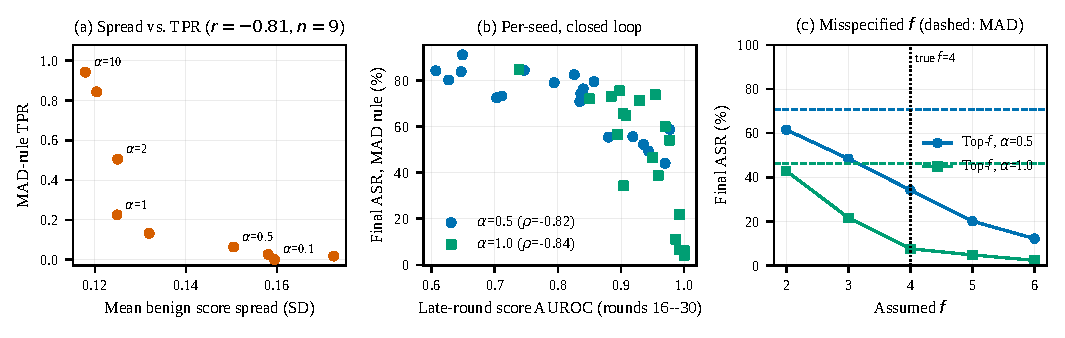
\includegraphics[width=\textwidth]{figs/fig_mech.pdf}
\caption{(a) Benign score spread against MAD-rule TPR across nine $\alpha$ values (Study A). (b) Per-seed late-round AUROC against final ASR of the MAD rule, closed loop, 20 seeds at each of two $\alpha$ (Study B). (c) Final ASR of the top-$f$ rule against assumed $f$ (true $f=4$) at 20 seeds; dashed lines show the MAD rule at the same $\alpha$.}
\label{fig:mech}
\end{figure*}

\subsection{What the Rank-Based Rule Gives, and What It Costs}
Replacing the MAD threshold by the top-$f$ rule lowers ASR sharply in the mid-range (Table~\ref{tab:b}): from 70.7\% to 34.2\% at $\alpha=0.5$ and from 46.4\% to 7.6\% at $\alpha=1$, with Holm-adjusted $p<0.001$ at both. The gain has three limits. (i) At $\alpha=0.5$ the result varies strongly across seeds (SD 30 points) and the interval is wide; the rule does not match an oracle threshold there. (ii) At $\alpha=0.1$ it does not help (85.4\%) and costs accuracy (76.0\% versus 81.2\%), with TPR 0.12 at FPR 0.22. (iii) It uses $f$, which is not generally known.

\label{sec:calib}Is the MAD rule simply mis-tuned? We swept its multiplier $k\in\{1,1.5,2\}$ ($\delta=0.1$) on all 20 Study B seeds and every $\alpha$, with top-$f$ ($f=4$) on the same scores. Lowering $k$ to 1 cuts ASR at $\alpha=0.5$ from 70.7\% to 43.6\% (top-$f$: 34.2\%) and at $\alpha=1$ from 46.4\% to 11.1\% (7.6\%); from $\alpha=2$ upward it matches top-$f$ without knowing $f$ (1.8\% vs.\ 1.5\% at $\alpha=2$, 0.7\% vs.\ 1.7\% at $\alpha=5$, 0.3\% vs.\ 0.8\% at $\alpha=10$). The paired gap between $k=1$ and top-$f$ is $+9.4$ points at $\alpha=0.5$ (Holm $p=0.008$) and $+3.5$ at $\alpha=1$ ($p=0.010$), so $k=1$ does not match the rank rule where heterogeneity is strongest. The price is false positives: FPR is 0.06--0.12 for $\alpha\ge0.5$ at $k=1$, against 0.01--0.06 at $k=2$, with clean accuracy within 0.4 points. At $\alpha=0.1$ no multiplier helps (86\% for every $k$). Much of the gap is therefore a calibration problem that a smaller fixed multiplier closes without $f$; $k=2$ had been picked from a coarse grid on three seeds, and $k=1$ is untested at CNN scale.

Misjudging $f$ (Fig.~\ref{fig:mech}c; 20 seeds, true $f=4$) matters in both directions. Assuming $f=2$ at $\alpha=1$ leaves ASR at 42.9\%, not distinguishable from the MAD rule (Holm $p=0.52$). Assuming $f=6$ lowers ASR further (2.3\% at $\alpha=1$) but raises FPR from 0.06 to 0.14, because benign clients are discarded; clean accuracy stays near 89\%, though discarding benign clients may cost more under data scarcity. Over-estimating $f$ is the safer error here.

\subsection{Probe-Aware Adaptive Attacker}\label{sec:adaptive}
We relax the threat model: malicious clients know that ProbeGuard is deployed, the probe bank, the scoring rule, and the global model. Each attacker minimises $\mathcal L_\text{backdoor}+\beta\,\mathcal L_\text{stealth}$, where the second term is a cross-entropy that pushes predictions on clean images patched at a random \emph{non-trigger} bank cell back to their true label. This penalises the bank-wide flip-rate elevation that drives the score while leaving the trigger cell itself untouched. We sweep $\beta\in\{0,0.1,0.25,0.5\}$ at $\alpha\in\{1,10\}$ on the 20 Study B seeds.

Stealth is not free for the attacker: raising $\beta$ lowers ASR against every defence, FedAvg included (69.6\%$\to$37.2\% at $\alpha=10$). Against top-$f$, however, ASR at $\alpha=1$ rises steadily with $\beta$ (7.3, 8.8, 10.7, 12.0\%; $\beta=0.5$ minus $\beta=0$ is $+4.8$ points, Wilcoxon $p=0.0015$) while TPR falls from 0.78 to 0.53; at $\alpha=10$ it stays at 1.9\% (Table~\ref{tab:adapt}). At $\alpha=1$ top-$f$ remains well below FedAvg (41.3\%) and the MAD rule (26.1\%) but is not distinguishable from Multi-Krum (10.1\%, $p=0.16$). Re-attacking the highest-flip-rate non-trigger cell each round did not noticeably raise ASR in a five-seed run (10.2\% versus 9.8\%). These are two strategies among many; a stronger optimiser cannot be ruled out.
\begin{table}[t]
\caption{Non-adaptive vs.\ adaptive attacker ($\beta{=}0.5$): ASR (\%), mean $\pm$ half-width of the 95\% bootstrap CI, 20 seeds.}
\label{tab:adapt}
\centering\footnotesize\setlength{\tabcolsep}{3pt}
\begin{tabular}{@{}lcccc@{}}
\toprule
 & \multicolumn{2}{c}{$\alpha=1$} & \multicolumn{2}{c}{$\alpha=10$}\\
\cmidrule(lr){2-3}\cmidrule(lr){4-5}
Defence & Non-adapt. & Adaptive & Non-adapt. & Adaptive\\
\midrule
FedAvg & 75.1$\pm$3.5 & 41.3$\pm$4.0 & 69.6$\pm$4.0 & 37.2$\pm$4.0\\
Multi-Krum & 43.2$\pm$14.2 & 10.1$\pm$4.5 & 9.5$\pm$9.0 & 5.8$\pm$4.5\\
MAD rule & 48.2$\pm$12.4 & 26.1$\pm$5.5 & 0.5$\pm$0.4 & 1.3$\pm$0.8\\
Top-$f$ rule & 7.3$\pm$6.7 & 12.0$\pm$4.1 & 0.8$\pm$0.7 & 1.9$\pm$1.0\\
\bottomrule
\end{tabular}
\end{table}

\subsection{CNN-Scale Check on CIFAR-10}
To see whether the probe score survives a larger model, we ran a CIFAR-10 experiment with a three-layer CNN (188,810 parameters): 20 clients, 20\% malicious, Dirichlet $\alpha=10$, a 200-image clean root set, 15 rounds, one local epoch per round (batch 32, SGD with learning rate 0.05 and momentum 0.9), and 8 seeds. The trigger is a $4{\times}4$ white patch in the bottom-right corner, and the probe bank is all $4{\times}4$ patches on a stride-4 grid (64 cells, including the trigger cell). The score uses all ten classes, and $k=2$, $\delta=0.1$ are carried over from the digits benchmark without re-tuning. Because of the compute budget, we ran only FedAvg, the two rules and the oracle, and the models are under-trained (about 54\% clean accuracy for every method), so ASR is read against the oracle's floor.
\begin{table}[t]
\caption{CIFAR-10 CNN, $\alpha=10$, 8 seeds: ASR (\%) with 95\% bootstrap interval, clean accuracy (\%), and cumulative client-level TPR/FPR.}
\label{tab:cnn}
\centering\footnotesize\setlength{\tabcolsep}{3.5pt}
\begin{tabular}{@{}lccc@{}}
\toprule
Defence & ASR [95\% CI] & Clean acc. & TPR/FPR\\
\midrule
FedAvg & 86.6 [85.5, 87.7] & 54.5 & --\\
MAD rule & 2.95 [2.08, 4.07] & 54.7 & 0.88/0.03\\
Top-$f$ rule & 2.82 [2.32, 3.47] & 54.6 & 0.91/0.02\\
Oracle & 2.45 [2.04, 2.90] & 54.3 & --\\
\bottomrule
\end{tabular}
\end{table}
Both rules end within about half a point of the oracle (Table~\ref{tab:cnn}): top-$f$ minus oracle is $+0.37$ points (Holm $p=0.50$), top-$f$ minus MAD is $-0.13$ points ($p=0.50$), and both are about 84 points below FedAvg ($p_\text{Holm}=0.031$, the smallest value an exact test can reach with eight seeds). Closed-loop score AUROC is 0.92 (MAD) and 0.91 (top-$f$) in rounds 1--5 and 0.998 and 1.000 in rounds 11--15. This matches the near-IID digits behaviour: with mild heterogeneity the score separates clients almost perfectly. We did not run $\alpha<10$ at CNN scale, so whether a fixed threshold degrades there is untested; the other baselines were not run.

\subsection{Cost and Component Checks}
ProbeGuard's probing roughly multiplies per-round wall-clock time by about 5.7 relative to FedAvg in our digits setup (34.7 ms versus 6.1 ms), against $+16\%$ to $+33\%$ for geometry-based baselines (the cost grows linearly with clients, bank size and root-set size, and our NumPy code is unoptimised); on the CNN, two rounds of the MAD rule took about 3.3 times as long as FedAvg (1,064 s versus 318 s, one CPU thread). In five-seed ablations at $\alpha=1$, top-$f$ ASR is 1.9--2.4\% for root sets of 25--100 images and 18.1\% (very wide interval) at 200, so a larger root set is not shown to help and probing cost could be cut, though we did not vary bank and root size jointly; with 4 probe cells top-$f$ reaches 12.8\%, against 0.6--2.8\% for 9 or more, while the MAD rule stays near 74\% throughout. Three alternative score definitions did not improve on the median reference at $\alpha=10$. With the fixed trigger, the largest flip rate falls on the trigger cell: peak 0.98 for malicious versus 0.38 for benign clients, so the score also localises the implanted patch.

\section{Discussion and Limitations}
The main lesson is methodological: a behavioural score can discriminate well while the tuned MAD rule and three percentile thresholds still fail under heterogeneity; a rank-based rule or a smaller MAD multiplier recovers much, not all, of the gap at mid-range $\alpha$. One fixed multiplier ($k=1$) holds up across $\alpha\ge0.75$ on digits; at CNN scale it is untested. Rules and scores should therefore be reported separately, with AUROC/AUPRC next to realised ASR. Limitations:
\begin{enumerate}
\item \emph{Scale.} The benchmark is $8{\times}8$ digits, a small MLP and 20 clients. The CIFAR-10 check covers only $\alpha=10$, eight seeds, one trigger and under-trained models (about 54\% clean accuracy), $k,\delta$ not re-tuned. We make no claim about realistic FL workloads.
\item \emph{Known $f$.} The top-$f$ rule needs the attacker count, as Multi-Krum does; we tested misspecification only for $f\in\{2,\dots,6\}$ with true $f=4$, and the malicious fraction was fixed at 20\% in Study B.
\item \emph{Adaptive attacker.} We tested one moderately tuned strategy and a variant (20 and 5 seeds), not an optimal search; top-$f$ degrades measurably under it at $\alpha=1$, and the results do not support a claim of robustness to adaptive adversaries.
\item \emph{Seed sets.} The open-loop AUROC, spread and ablation analyses use other seeds and protocols (5--8 seeds) than Study B, and their AUROC values differ from the closed-loop ones. Three of the 20 Study-B seeds were used to tune the MAD parameters.
\item \emph{Baselines} are simplified re-implementations; the spread--TPR correlation ($n=9$) is not causal evidence.
\item \emph{Triggers.} Only four patch-type triggers were tested; distributed, non-patch and learned triggers were not.
\item \emph{Overhead.} Probing costs 3--6 times FedAvg's per-round time and did not help at $\alpha\le0.25$ here.
\end{enumerate}

\section{Conclusion}
Behavioural trigger probing detects backdoors well on near-IID data and localises the trigger, but with a fixed threshold it degrades under strong heterogeneity although its scores stay informative at moderate levels. On a controlled benchmark with 20 seeds, a rank-based rule recovers most of the loss for $\alpha$ between 0.75 and 2 and part of it at $\alpha=0.5$, and a smaller MAD multiplier does as well from $\alpha=2$ upward and within 3.5--9.4 points at $\alpha=0.5$--1 (20 seeds), at the price of false positives (and, for the rank rule, of needing $f$); it does not help at $\alpha=0.1$, and coordinate median and FLTrust stay better there. A CIFAR-10 CNN check at $\alpha=10$ shows both rules close to an oracle with near-perfect score separation, but it says nothing yet about heterogeneity at that scale. The results support cautious optimism about decision-rule design for behavioural defences, not a deployable defence. Future work: the CNN study at $\alpha\le1$ with more seeds and baselines, optimiser-based adaptive attackers, unknown $f$, comparison with recent model-inspection defences, and heterogeneity-aware thresholds.

\textit{Reproducibility.} Code, per-run results and unit tests are at \texttt{github.com/mihiit/Backdoorfed-ICTACS}; the digits runs are deterministic NumPy and the dataset ships with scikit-learn. \textit{Acknowledgment.} The authors thank the anonymous reviewers for their comments.

\begin{thebibliography}{99}
\bibitem{mcmahan2017} H. B. McMahan, E. Moore, D. Ramage, S. Hampson, and B. A. y Arcas, ``Communication-efficient learning of deep networks from decentralized data,'' in \emph{Proc. AISTATS}, PMLR vol.~54, 2017, pp. 1273--1282.
\bibitem{li2025survey} Z. Li, J. Lan, Z. Yan, and E. Gelenbe, ``Backdoor attacks and defense mechanisms in federated learning: A survey,'' \emph{Information Fusion}, vol.~123, Art.~103248, 2025.
\bibitem{blanchard2017} P. Blanchard, E. M. El Mhamdi, R. Guerraoui, and J. Stainer, ``Machine learning with adversaries: Byzantine tolerant gradient descent,'' in \emph{Proc. NeurIPS}, vol.~30, 2017.
\bibitem{yin2018} D. Yin, Y. Chen, K. Ramchandran, and P. Bartlett, ``Byzantine-robust distributed learning: Towards optimal statistical rates,'' in \emph{Proc. ICML}, PMLR vol.~80, 2018, pp. 5650--5659.
\bibitem{cao2021} X. Cao, M. Fang, J. Liu, and N. Z. Gong, ``FLTrust: Byzantine-robust federated learning via trust bootstrapping,'' in \emph{Proc. NDSS}, 2021.
\bibitem{rieger2022} P. Rieger, T. D. Nguyen, M. Miettinen, and A.-R. Sadeghi, ``DeepSight: Mitigating backdoor attacks in federated learning through deep model inspection,'' in \emph{Proc. NDSS}, 2022.
\bibitem{nguyen2022} T. D. Nguyen \emph{et al.}, ``FLAME: Taming backdoors in federated learning,'' in \emph{Proc. 31st USENIX Security Symp.}, 2022, pp. 1415--1432.
\bibitem{rieger2024} P. Rieger, T. Krau{\ss}, M. Miettinen, A. Dmitrienko, and A.-R. Sadeghi, ``CrowdGuard: Federated backdoor detection in federated learning,'' in \emph{Proc. NDSS}, 2024, doi: 10.14722/ndss.2024.23233.
\bibitem{zhang2025} X. Zhang \emph{et al.}, ``Runtime backdoor detection for federated learning via representational dissimilarity analysis,'' \emph{arXiv:2503.04473}, 2025.
\bibitem{xu2024} X. Xu, K. Huang, Y. Li, Z. Qin, and K. Ren, ``Towards reliable and efficient backdoor trigger inversion via decoupling benign features,'' in \emph{Proc. ICLR}, 2024.
\bibitem{li2022niid} Q. Li, Y. Diao, Q. Chen, and B. He, ``Federated learning on non-IID data silos: An experimental study,'' in \emph{Proc. IEEE ICDE}, 2022.
\bibitem{fereidooni2024} H. Fereidooni, A. Pegoraro, P. Rieger, A. Dmitrienko, and A.-R. Sadeghi, ``FreqFed: A frequency analysis-based approach for mitigating poisoning attacks in federated learning,'' in \emph{Proc. NDSS}, 2024, doi: 10.14722/ndss.2024.23620.
\bibitem{huang2023} T. Huang \emph{et al.}, ``Lockdown: Backdoor defense for federated learning with isolated subspace training,'' in \emph{Proc. NeurIPS}, vol.~36, 2023.
\bibitem{xu2025} J. Xu, Z. Zhang, and R. Hu, ``Detecting backdoor attacks in federated learning via direction alignment inspection,'' in \emph{Proc. IEEE/CVF CVPR}, 2025.
\bibitem{yang2025} Y. Yang \emph{et al.}, ``FilterFL: Knowledge filtering-based data-free backdoor defense for federated learning,'' in \emph{Proc. ACM CCS}, 2025.
\bibitem{pedregosa2011} F. Pedregosa \emph{et al.}, ``Scikit-learn: Machine learning in Python,'' \emph{J. Mach. Learn. Res.}, vol.~12, pp. 2825--2830, 2011.
\bibitem{harris2020} C. R. Harris \emph{et al.}, ``Array programming with NumPy,'' \emph{Nature}, vol.~585, pp. 357--362, 2020.
\bibitem{virtanen2020} P. Virtanen \emph{et al.}, ``SciPy 1.0: Fundamental algorithms for scientific computing in Python,'' \emph{Nature Methods}, vol.~17, pp. 261--272, 2020.
\end{thebibliography}
